\subsection{}
Oligopolies have 5 assumptions:
\begin{enumerate}
    \item Price makers.
    \item Many buyers and few sellers.
    \item Heterogeneous product (differentiated).
    \item Barriers to entry and exit.
    \item Imperfect information.
\end{enumerate}
Examples of oligopolies are Canadian banking industry.\\
Two firms in an oligopoly is called a duopoly.
\par
Strategic interdependence is when firms are aware of the actions of other firms and take that into account when making decisions.\\
Game theory is used to analyze the strategic interactions between firms.\\
A payoff matrix is a table that shows the payoffs for every possible action by each player.\\
We will look at an example with two firms and two strategies.\\
Firm B has the ability to announce to cooperate with firm A or compete.\\
Firm A has the ability to cooperate with firm B or compete.\\
A dominant strategy is a strategy that is best for a player in a game regardless of the strategies chosen by the other players.
Nash equilibrium is that the players do not want to change their strategy after it has been chosen.
\begin{figure}[H]
    \centering
    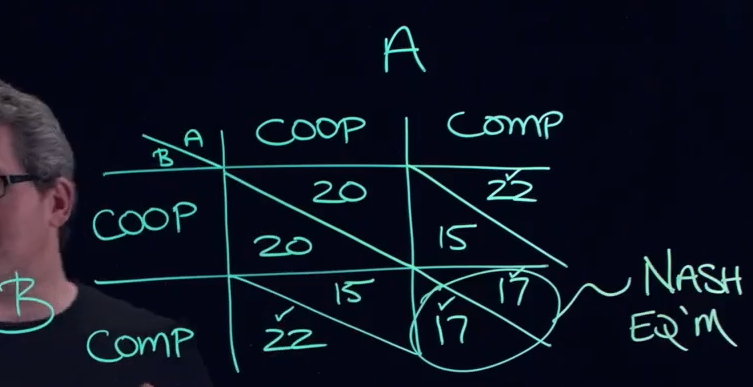
\includegraphics[width=0.5\textwidth]{Chapter11/GameTheory.png}
    \caption{Game Theory}
    \label{fig:gametheory}
\end{figure}
In this example, the Nash equilibrium is for both firms to compete (compete-compete).